%% LyX 2.2.1 created this file.  For more info, see http://www.lyx.org/.
%% Do not edit unless you really know what you are doing.
\documentclass[english,12pt]{article}
\usepackage[T1]{fontenc}
\usepackage[latin9]{inputenc}
\usepackage{prettyref}
\usepackage{amsmath}
\usepackage{amsthm}
\usepackage{amssymb}
\usepackage{graphicx}

\makeatletter
%%%%%%%%%%%%%%%%%%%%%%%%%%%%%% Textclass specific LaTeX commands.
\theoremstyle{plain}
\newtheorem{thm}{\protect\theoremname}[section]
\theoremstyle{definition}
\newtheorem{defn}[thm]{\protect\definitionname}
\theoremstyle{plain}
\newtheorem{prop}[thm]{\protect\propositionname}
\ifx\proof\undefined
\newenvironment{proof}[1][\protect\proofname]{\par
\normalfont\topsep6\p@\@plus6\p@\relax
\trivlist
\itemindent\parindent
\item[\hskip\labelsep\scshape #1]\ignorespaces
}{%
\endtrivlist\@endpefalse
}
\providecommand{\proofname}{Proof}
\fi
\theoremstyle{definition}
\newtheorem{example}[thm]{\protect\examplename}
\theoremstyle{plain}
\newtheorem{cor}[thm]{\protect\corollaryname}
\theoremstyle{definition}
\newtheorem{xca}[thm]{\protect\exercisename}

%%%%%%%%%%%%%%%%%%%%%%%%%%%%%% User specified LaTeX commands.
\usepackage[margin=1in]{geometry}

\newrefformat{prop}{Proposition \ref{#1}}
\newrefformat{exa}{Example \ref{#1}}

\makeatother

\usepackage{babel}
\providecommand{\corollaryname}{Corollary}
\providecommand{\definitionname}{Definition}
\providecommand{\examplename}{Example}
\providecommand{\exercisename}{Exercise}
\providecommand{\propositionname}{Proposition}
\providecommand{\theoremname}{Theorem}

\begin{document}

\title{Math 525: Lecture 2}

\date{January 9, 2018}

\maketitle

For the entirety of this lecture, we will always assume an underlying
probability space $(\Omega,\mathcal{F},\mathbb{P})$. Recall that
$\mathcal{F}$ is a $\sigma$-algebra on $\Omega$ and $\mathbb{P}\colon\mathcal{F}\rightarrow[0,1]$
is a probability measure.

\section{Conditional probability}
\begin{defn}
We say $A\in\mathcal{F}$ is a \emph{null event} (or simply \emph{null})
if $\mathbb{P}(A)=0$.
\end{defn}
Given $A,C\in\mathcal{F}$ such that $C$ is not null, how do we define
the ``probability of $A$ given $C$''? Let's do a thought experiment.
If $A$ and $C$ are two (possibly overlapping) regions of a dartboard,
we may throw $N$ darts at a dart board and count $n(A\cap C)$, the
number of darts which land in $A\cap C$ and $n(C)$, the number of
darts which land in $C$. Now, let $\mathbb{P}(A\mid C)$ denote the
probability that a dart lands in region $A$ given that it lands in
region $C$ and $\mathbb{P}(X)$ denote the probability that it lands
in region $X$. Then, at least intuitively,
\[
\mathbb{P}(A\mid C)=\lim_{N\rightarrow\infty}\frac{n(A\cap C)}{n(C)}=\lim_{N\rightarrow\infty}\frac{\frac{n(A\cap C)}{N}}{\frac{n(C)}{N}}=\frac{\mathbb{P}(A\cap C)}{\mathbb{P}(C)}.
\]
This suggest the following definition of condition probability.
\begin{defn}
Let $A,C\in\mathcal{F}$ such that $C$ is not null. The \emph{conditional
probability of $A$ given $C$} is defined as
\[
\mathbb{P}(A\mid C)=\frac{\mathbb{P}(A\cap C)}{\mathbb{P}(C)}.
\]
Equivalently, the conditional probability $\mathbb{P}(A\mid C)$ is
the unique number satisfying
\begin{equation}
\mathbb{P}(A\mid C)\mathbb{P}(C)=\mathbb{P}(A\cap C).\label{eq:conditional_probability_rearrangement}
\end{equation}
\end{defn}
\begin{prop}[Bayes' Rule]
Let $B_{1},\ldots,B_{n}\in\mathcal{F}$ be a partition of $\Omega$
such that each $B_{i}$ is not null. Then, for any non-null $A\in\mathcal{F}$,
\[
\mathbb{P}(B_{j}\mid A)=\frac{\mathbb{P}(A\mid B_{j})\mathbb{P}(B_{j})}{\sum_{i}\mathbb{P}(A\mid B_{i})\mathbb{P}(B_{i})}=\left(1+\frac{\sum_{i\neq j}\mathbb{P}(A\mid B_{i})\mathbb{P}(B_{i})}{\mathbb{P}(A\mid B_{j})\mathbb{P}(B_{j})}\right)^{-1}.
\]
\end{prop}
\begin{proof}
The proof is just two applications of \eqref{eq:conditional_probability_rearrangement}:
\[
\mathbb{P}(B_{j}\mid A)=\frac{\mathbb{P}(B_{j}\cap A)}{\mathbb{P}(A)}=\frac{\mathbb{P}(A\mid B_{j})\mathbb{P}(B_{j})}{\sum_{i}\mathbb{P}(A\cap B_{j})}=\frac{\mathbb{P}(A\mid B_{j})\mathbb{P}(B_{j})}{\sum_{i}\mathbb{P}(A\mid B_{i})\mathbb{P}(B_{i})}.\qedhere
\]
\end{proof}
A famous example in which conditional probability produces unexpected
results is the Monty Hall Problem:
\begin{example}[Monty Hall Problem]
Suppose you're on a game show, and you're given the choice of three
doors: Behind one door is a car; behind the others, goats. You pick
a door, say No. 1, and the host, who knows what's behind the doors,
opens \textbf{another} door, say No. 3, which has a goat. He then
says to you, ``Do you want to pick door No. 2?'' Is it to your advantage
to switch your choice?

\begin{figure}
\begin{centering}
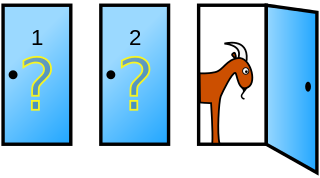
\includegraphics[scale=0.5]{monty_hall}
\par\end{centering}
\caption{Monty Hall Problem}
\end{figure}

There are some things to keep in mind before you make your choice:
\begin{itemize}
\item The car is just as likely to be behind door No. $1$ as it is to be
behind any other door (as such, we may as well always assume you initially
choose door No. 1).
\item Once you have made your initial choice, the host will not choose to
open your door. Moreover, the host will not open the door with the
car behind it.
\end{itemize}
Let $C_{i}$ be the event that the car is behind door No. $i$. We
have $\mathbb{P}(C_{i})=1/3$. Let $H$ be the event that the host
chooses door No. 3. We have,
\begin{align*}
\mathbb{P}(H\mid C_{1}) & =1/2\\
\mathbb{P}(H\mid C_{2}) & =1\\
\mathbb{P}(H\mid C_{3}) & =0.
\end{align*}
By Bayes' rule,
\[
\mathbb{P}(C_{2}\mid H)=\left(1+\frac{\mathbb{P}(H\mid C_{1})\mathbb{P}(C_{1})+\mathbb{P}(H\mid C_{3})\mathbb{P}(C_{3})}{\mathbb{P}(H\mid C_{2})\mathbb{P}(C_{2})}\right)^{-1}=\frac{1}{1+1/2}=\frac{2}{3}.
\]
It is in your best interests to \textbf{switch} doors!
\end{example}

\section{Independence}
\begin{defn}
Let $A,B\in\mathcal{F}$. We say $A$ and $B$ are \emph{independent}
if
\[
\mathbb{P}(A\cap B)=\mathbb{P}(A)\mathbb{P}(B).
\]
\end{defn}
The definition of independence is motivated by the following observation:
\begin{prop}
\label{prop:independence}Let $A,B\in\mathcal{F}$ with $B$ not null.
Then, $A$ and $B$ are independent if and only if $\mathbb{P}(A\mid B)=\mathbb{P}(A)$.
\end{prop}
\begin{proof}
Suppose $A$ and $B$ are independent. Then, 
\[
\mathbb{P}(A\mid B)=\frac{\mathbb{P}(A\cap B)}{\mathbb{P}(B)}=\frac{\mathbb{P}(A)\mathbb{P}(B)}{\mathbb{P}(B)}=\mathbb{P}(A).
\]
Suppose now that $\mathbb{P}(A\mid B)=\mathbb{P}(A)$. Then,
\[
\mathbb{P}(A\cap B)=\mathbb{P}(A\mid B)\mathbb{P}(B)=\mathbb{P}(A)\mathbb{P}(B).\qedhere
\]
\end{proof}
Note that if at least one of $A$ and $B$ are null, then $A$ and
$B$ are trivially independent. For example, if $B$ is null, we have
\[
\mathbb{P}(A\cap B)\leq\mathbb{P}(B)=0.
\]
Since $\mathbb{P}(\cdot)\geq0$, it follows that $\mathbb{P}(A\cap B)=0$.
\begin{cor}
Let $A,B\in\mathcal{F}$ be non-null. Then, 
\[
\mathbb{P}(A\mid B)=\mathbb{P}(A)\iff\mathbb{P}(B\mid A)=\mathbb{P}(B)
\]
\end{cor}
\begin{proof}
If $\mathbb{P}(A\mid B)=\mathbb{P}(A)$, then $A$ and $B$ are independent.
Reversing the roles of $A$ and $B$ in \prettyref{prop:independence},
we obtain $\mathbb{P}(B\mid A)=\mathbb{P}(B)$.
\end{proof}

\section{Counting}

In this section, we review some basic facts about counting that you
may have previously encountered in a combinatorics class.
\begin{defn}
A \emph{permutation} of a (possibly finite) sequence of elements is
simply a reordering of that sequence.
\end{defn}
\begin{example}
The sequence $(a,b,c)$ has 6 permutations: $(a,b,c)$, $(a,c,b)$,
$(b,a,c)$, $(b,c,a)$, $(c,a,b)$, $(c,b,a)$. 
\end{example}
Given a sequence $(1,\ldots,n)$ with $n$ elements, we want to determine
the number of permutations $(i_{1},\ldots,i_{n})$. We argue as follows:
to pick the first item $i_{1}$ in the permutation, we have $n$ items
available to us. Once we have picked the first item, we have $n-1$
options for the second item $i_{2}$, and so forth. Therefore, there
are
\[
n\left(n-1\right)\left(n-2\right)\cdots1\equiv\boxed{n!}
\]
permutations of a sequence with $n$ elements.
\begin{xca}
We have an urn with $n$ \textbf{distinct} balls. We first pull out
a ball and set it down. We next pull out another ball and place it
to the right of the first ball, and continue in this way until we
have $r\le n$ balls in a row:
\[
b_{1}\quad b_{2}\quad\cdots\quad b_{r}
\]
There are exactly
\[
n\left(n-1\right)\left(n-2\right)\cdots\left(n-r+1\right)=\boxed{\frac{n!}{\left(n-r\right)!}}
\]
ways we can do this.
\end{xca}
The above is referred to as sampling \textbf{without replacement},
since we do not return a ball to the urn after having drawn it. If
we are sampling \textbf{with replacement}, we would have $\boxed{n^{r}}$
possibilities. What if we sample \textbf{without replacement, but
without regards to order}? That is, how many ways are there to \emph{choose}
$r$ objects out of $n$ distinct ones? Since there are $r!$ permutations
of a sequence of $r$ objects, this is simply
\[
\frac{\text{\# of ways to sample }r\text{ objects from }n\text{ w/o replacement}}{\text{\# of ways to permute }r\text{ objects}}=\frac{1}{r!}\frac{n!}{\left(n-r\right)!}\equiv\boxed{\binom{n}{r}}.
\]


\section{Linear homogeneous recurrence relations (optional)}

This section reviews linear homogeneous recurrence relations, which
are used in the example in the next section involving the gambler's
ruin. This material is mostly for your interest, and won't be tested.

Consider the equation
\begin{equation}
a_{n}+c_{1}a_{n-1}+\cdots+c_{d}a_{n-d}=0\label{eq:recurrence}
\end{equation}
where $c_{1},\ldots,c_{d}$ are (real or complex) constants. This
is called a \emph{linear homogeneous recurrence relation}. A solution
of this equation is a sequence $(a_{n})_{n\geq1}$ that satisfies
it. How do we find the solutions?

Let's proceed by guessing that a solution is of the form
\[
a_{n}=r^{n}
\]
where $r\neq0$. Indeed, if this is the case, \eqref{eq:recurrence}
suggests that
\[
r^{n}+c_{1}r^{n-1}+\cdots+c_{d}r^{n-d}=0.
\]
Multiplying both sides of the above by $r^{d-n}$, 
\begin{equation}
r^{d}+c_{1}r^{d-1}+\cdots+c_{d}r^{0}=0\label{eq:characteristic_polynomial}
\end{equation}
(note that $r^{0}=1$). The quantity on the left hand side of the
equation \eqref{eq:characteristic_polynomial} is called the \emph{characteristic
polynomial} associated with the recurrence.

By the fundamental theorem of algebra, the characteristic polynomial
has $d$ roots, which we label $r_{1},\ldots,r_{d}$. By the argument
in the previous paragraph, for any $1\leq i\leq d$, defining the
sequence $(a_{n})_{n\geq1}$ by 
\[
a_{n}=r_{i}^{n}
\]
yields a solution of the recurrence.

In fact, we can do even better than that. If we assume that the roots
are distinct (i.e., $r_{i}\neq r_{j}$ whenever $i\neq j$), then
the sequence $(a_{n})_{n\geq1}$ defined by 
\[
a_{n}=C_{1}r_{1}^{n}+\cdots+C_{d}r_{d}^{n}
\]
is also a solution of the recurrence, where $C_{1},\ldots,C_{d}$
are arbitrary (real or complex) constants.

\section{Gambler's ruin (optional)}

Consider a gambler who repeatedly plays a game against an opponent
in which they receive a dollar with probability $p$ and lose a dollar
with probability $1-p$. Both the gambler and their opponent start
off with initial stakes of $n$ and $m$ dollars, respectively. The
game ends when either the gambler or the opponent are broke.

Let $N=n+m$ be the total amount of money in the game. Let
\[
f(k)=\mathbb{P}(\text{Gambler goes broke if initial stake is }k).
\]
If the gambler has no money left, the game ends with the gambler broke.
Therefore, $f(0)=1$. The game also ends if the gambler has all the
money in the game. Therefore, $f(N)=0$. Moreover,
\[
f(k)=pf(k+1)-\left(1-p\right)f(k-1)\qquad\text{if }0<k<N.
\]
We rewrite the above as
\[
\boxed{f(k+1)-\frac{1}{p}f(k)+\left(\frac{1}{p}-1\right)f(k-1)=0\qquad\text{if }0<k<N}.
\]
Ignoring the quantifier ``if $0<k<N$'', the above becomes
\[
f(k+1)-\frac{1}{p}f(k)+\left(\frac{1}{p}-1\right)f(k-1)=0.
\]
This is nothing other than a linear homogeneous recurrence relation!
Its characteristic polynomial is
\[
r^{2}-\frac{1}{p}r+\left(\frac{1}{p}-1\right)r,
\]
which has roots $1$ and $a=\frac{1}{p}-1$. Assuming $p\neq\frac{1}{2}$,
the roots are distinct, and we can use the strategy of the previous
section to conclude that a solution of this recurrence is
\begin{equation}
f(k)=A+Ba^{k}\label{eq:general_solution}
\end{equation}
where $A$ and $B$ are arbitrary real constants. To determine the
specific value of the constants $A$ and $B$, we employ the boundary
conditions. Namely,
\[
f(0)=1=A+B\qquad\text{and}\qquad f(N)=0=A+Ba^{N}.
\]
If we solve the above equations for $A$ and $B$, we get
\[
A=-\frac{a^{N}}{1-a^{N}}\qquad\text{and}\qquad B=\frac{1}{1-a^{N}}.
\]
Plugging the above back into \eqref{eq:general_solution}, we get
\[
\boxed{f(k)=\frac{a^{k}-a^{N}}{1-a^{N}}\qquad\text{if }0\leq k\leq N}.
\]
Recall that our calculations were only accurate in the case of $p\neq\frac{1}{2}$.
If $p=\frac{1}{2}$ (equivalently, $a=1$), we can take limits to
obtain the answer. By L'Hopital's rule,
\[
\lim_{a\rightarrow1}f(k)=\lim_{a\rightarrow1}\frac{a^{n}-a^{N}}{1-a^{N}}=\lim_{a\rightarrow1}a^{n}\frac{1-a^{N-n}}{1-a^{N}}=\lim_{a\rightarrow1}\frac{1-a^{N-n}}{1-a^{N}}=\frac{N-n}{N}.
\]


\section{Generating a $\sigma$-algebra and Borel sets}

Often times, we only have a small set of events $\mathcal{G}$ that
do not necessarily form a $\sigma$-algebra. Since the probabilistic
framework requires a $\sigma$-algebra, we need a procedure to ``generate''
a $\sigma$-algebra from $\mathcal{G}$.
\begin{defn}
Let $\mathcal{G}\subset2^{\Omega}$ be a set. Then, the \emph{$\sigma$-algebra
generated from $\mathcal{G}$} is
\[
\sigma(\mathcal{G})=\bigcap_{\substack{\mathcal{F}\text{ is a }\sigma\text{-algebra on }\Omega\\
\mathcal{G}\subset\mathcal{F}
}
}\mathcal{F}.
\]
\end{defn}
In the first assignment, you are asked to prove the following:
\begin{prop}
$\sigma(\mathcal{G})$ is the ``smallest'' $\sigma$-algebra on
$\Omega$ which contains $\mathcal{G}$. That is, for any $\sigma$-algebra
$\mathcal{F}$ satisfying $\mathcal{G}\subset\mathcal{F}$, it follows
that $\sigma(\mathcal{G})\subset\mathcal{F}$.
\end{prop}
In the previous lecture, we mentioned that in the case of a countable
sample space $\Omega$, we could simply take the $\sigma$-algebra
to be the powerset (i.e., $\mathcal{F}=2^{\Omega})$. In this case,
any probability space has the form $(\Omega,2^{\Omega},\mathbb{P})$.
Recall that in the case of an uncountable sample space $\Omega$,
this approach fails. In this case, however, we can often take the
$\sigma$-algebra $\mathcal{F}$ to be the something called the Borel
$\sigma$-algebra. Let's first discuss what the Borel $\sigma$-algebra
is in the case of $\Omega=\mathbb{R}$, generalizing later to metric
and topological spaces.
\begin{defn}
Let
\[
\mathcal{G}=\left\{ (-\infty,x]\colon x\in\mathbb{R}\right\} 
\]
be the set of all intervals of the form $(-\infty,x]$. Note that
$\mathcal{G}\subset2^{\mathbb{R}}$. Let $\mathcal{B}(\mathbb{R})=\sigma(\mathcal{G})$.
We call $\mathcal{B}(\mathbb{R})$ the \emph{Borel $\sigma$-algebra}
on $\mathbb{R}$, and refer to any element of $\mathcal{B}(\mathbb{R})$
as a Borel set.
\end{defn}
\begin{example}
Any open interval is a Borel set. To see this, let $(a,b)$ be an
open interval with $a<b$. First, note that
\[
\bigcup_{n\geq1}(-\infty,b-1/n]=(-\infty,b).
\]
Therefore,
\[
(-\infty,a]^{c}\cap\left(-\infty,b\right)=(a,b)
\]
and hence $(a,b)\in\mathcal{B}(\mathbb{R})$. A similar argument yields
that any closed interval $[a,b]$ with $a<b$ is also a Borel set.
\end{example}
%
\begin{example}
\label{exa:countable_union}Any open set is a Borel set. This is a
direct consequence of the fact that any open set $G\subset\mathbb{R}$
is a countable union of open intervals $G=\cup_{n\geq1}(a_{n},b_{n})$.
Moreover, since a closed set $F$ is a complement of an open set $F=G^{c}$,
any closed set is also a Borel set (remember, the Borel $\sigma$-algebra
is closed under complements).
\end{example}

\section{Generalizing the Borel sets (optional)}

\prettyref{exa:countable_union} implies that we could have also defined
the Borel sets on $\mathbb{R}$ by
\[
\mathcal{B}(\mathbb{R})=\sigma(\left\{ G\subset\mathbb{R}\colon G\text{ is open}\right\} ).
\]
This suggests that we can generalize Borel sets to metric spaces (or
even more generally, topological spaces):
\begin{defn}[Borel sets on metric spaces]
Let $(X,d)$ be a metric space. Then,
\[
\mathcal{B}(X)=\sigma(\left\{ G\subset X\colon G\text{ is open with respect to }d\right\} )
\]
is the set of Borel sets on $X$.
\end{defn}
%
\begin{defn}[Borel sets on topological spaces]
Let $(X,\tau)$ be a topological space. Then,
\[
\mathcal{B}(X)=\sigma(\left\{ G\subset X\colon G\in\tau\right\} )
\]
is the set of Borel sets on $X$.
\end{defn}

\end{document}
